\documentclass[border=10pt]{standalone}

\usepackage{tikz}
\usepackage{tikzsymbols}
\usetikzlibrary{calc,patterns,shapes.geometric}

\def\centerarc[#1](#2)(#3:#4:#5){\draw[#1] ($(#2)+({#5*cos(#3)},{#5*sin(#3)})$) arc (#3:#4:#5);}

\begin{document}
	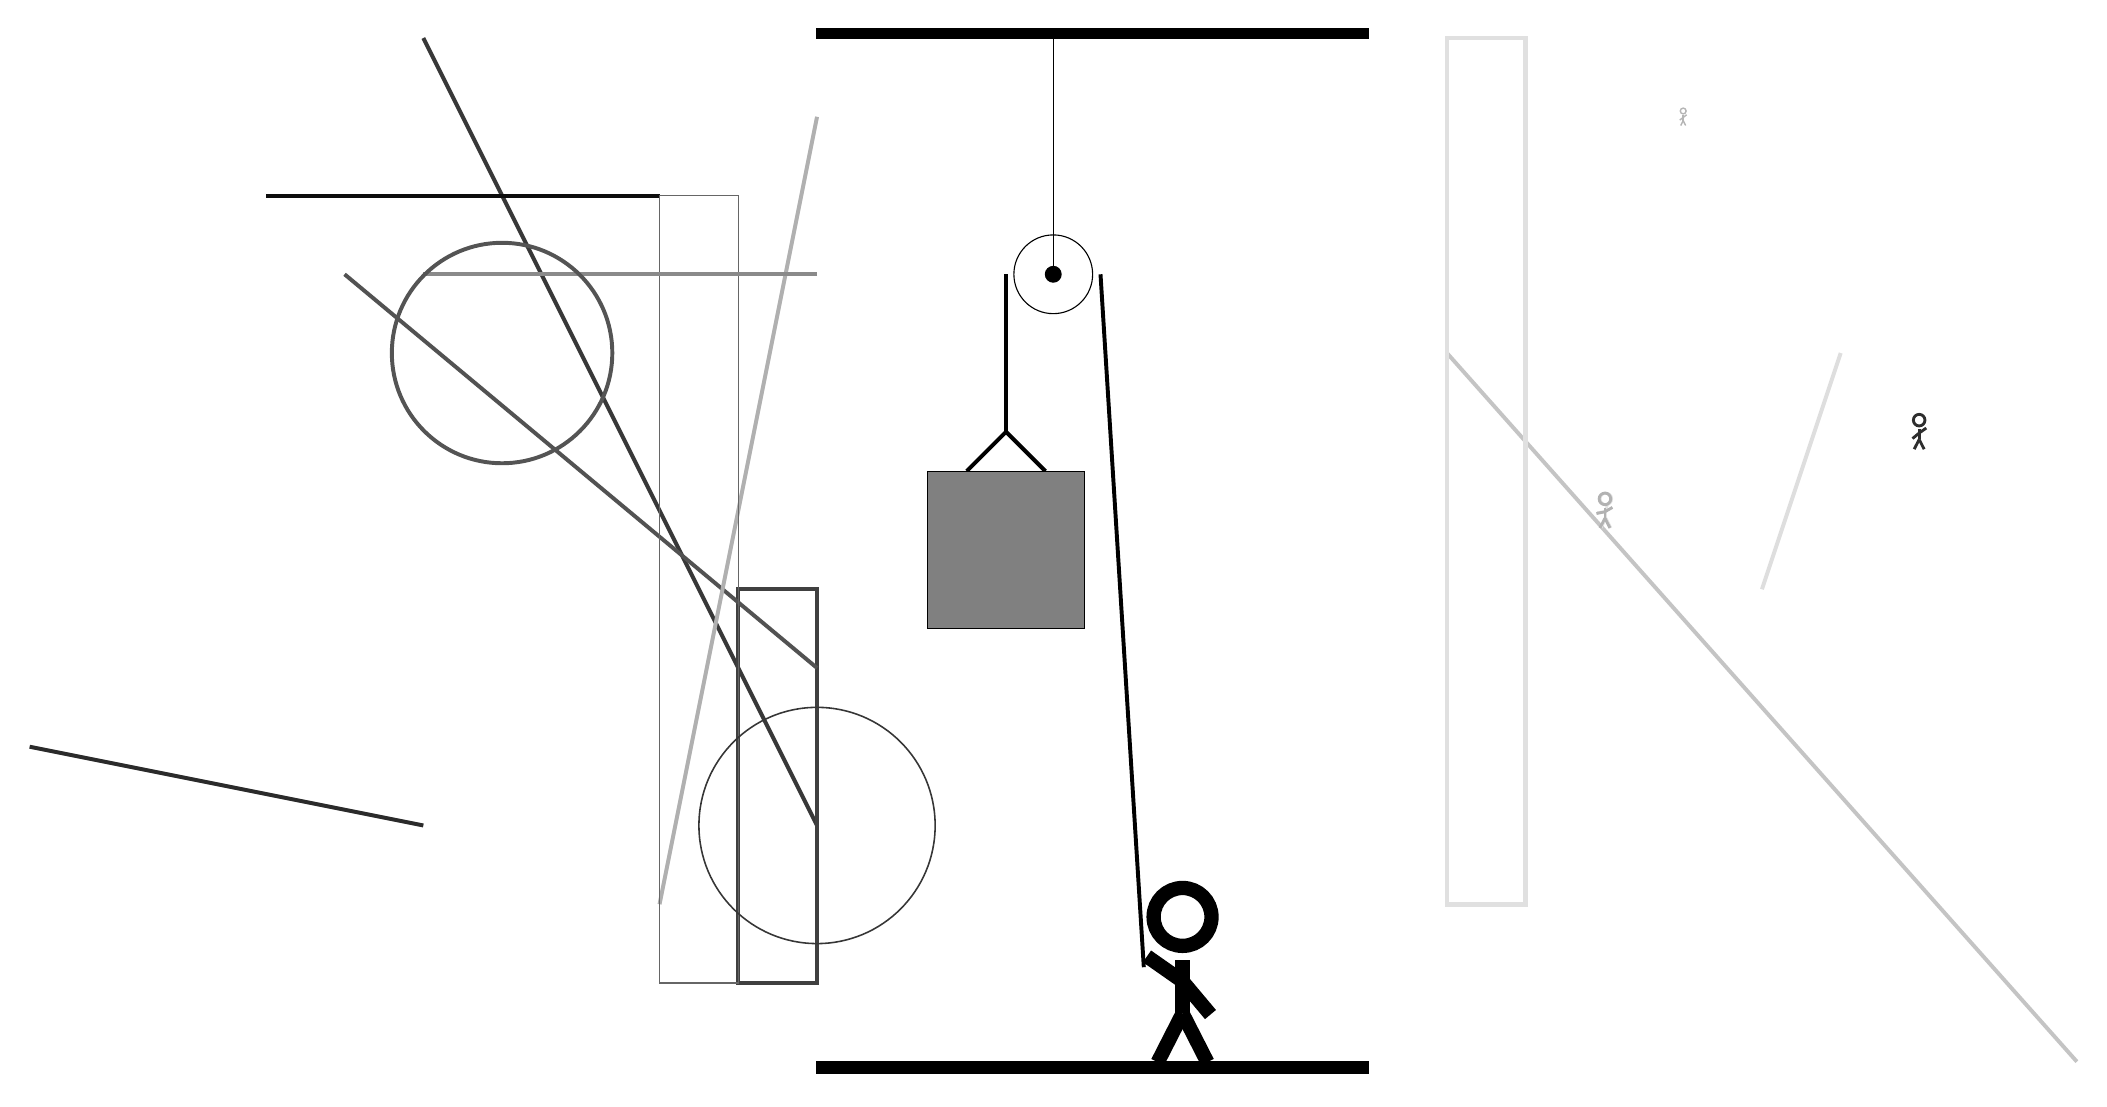
\begin{tikzpicture}
		%%%%% START %%%%%
		
		\draw[fill=black] (-2, 10) rectangle (5, 10.125);
		
		\draw (1, 7) circle (0.5);
		\draw[fill=black] (1, 7) circle (0.1);
		\draw (1, 10) -- (1, 7);
		
		\draw[line width=0.5mm] (-0.1, 4.5) -- (0.4, 5.0) -- (0.9, 4.5);
		\draw[fill=black!50] (-0.6, 4.5) rectangle (1.4, 2.5);
		
		\draw[line width=0.5mm] (0.4, 7) -- (0.4, 5.0);
		\centerarc[line width=0.5mm](1, 7)(0:180:0.6);
		\draw[line width=0.5mm](1.6, 7) -- (2.15, -1.8);
		
		\node at (2.6, -1.9) {\Strichmaxerl[10][-35][-50]};
		
		\draw[line width=0.5mm, color=black!78](-7, 10) -- (-2, 0);
		
		\draw[line width=0.5mm, color=black!75] (-2, -2) rectangle (-3, 3);
		\draw[line width=0.5mm, color=black!83](-7, 0) -- (-12, 1);
		\draw[line width=0.5mm, color=black!23](6, 6) -- (14, -3);
		\node[line width=0.2mm, color=black!29] at (9, 9) {\Strichmaxerl[1][37][38]};
		\draw[line width=0.6mm, color=black!12] (6, -1) rectangle (7, 10);
		
		\node[line width=0.5mm, color=black!11] at (8, 4) {\Strichmaxerl[2][6][79]};
		\draw[line width=0.5mm, color=black!95](-4, 8) -- (-9, 8);
		\node[line width=0.7mm, color=black!82] at (12, 5) {\Strichmaxerl[2][40][35]};
		\node[line width=0.7mm, color=black!30] at (8, 4) {\Strichmaxerl[2][12][30]};
		\draw[line width=0.5mm, color=black!68](-2, 2) -- (-8, 7);
		\draw[line width=0.5mm, color=black!31](-4, -1) -- (-2, 9);
		\draw[line width=0.2mm, color=black!60] (-3, 8) rectangle (-4, -2);
		
		\draw [line width=0.2mm, color=black!79](-2, 0) circle (1.5);
		\draw[line width=0.5mm, color=black!13](10, 3) -- (11, 6);
		\draw[line width=0.5mm, color=black!46](-2, 7) -- (-7, 7);
		
		\draw [line width=0.5mm, color=black!67](-6, 6) circle (1.4);
		
		\draw[fill=black] (-2, -3) rectangle (5, -3.15);
		
		%%%%% END %%%%%
	\end{tikzpicture}
\end{document}